\chapter{Introducción}

\section{Motivación y antecedentes}

A partir de los años 90 Internet tuvo una gran expansión, pasando de solo compartir información entre investigadores, 
como se hacía al principio, a permitir realizar compras, hacer videollamadas, pedir cita en el médico, gestionar 
todo lo relacionado con el banco y demás. Internet 
llega a miles de millones de personas que consumen recursos de forma masiva. Por lo que es crucial tener cierta 
calidad de servicio en los recursos que se consumen.

\intro La calidad de servicio es lo más importante tanto a nivel de desarrollo como de consumidor. Como desarrollador, 
se tendrá que pensar en esta característica como una de las más importantes, pues un mal servicio hará que se pierdan 
clientes. Como cliente la calidad de servicio es algo deseable, pues si por ejemplo en un servicio de videollamada se 
experimenta cierta perdida de calidad, no pasará nada. Por el contrario si en un servicio de visionado de contenido 
bajo demanda de algún evento deportivo se experimenta la perdida de calidad en la imagen o se cae el servicio lo más 
probable es que el usuario que lo experimenta no vuelva a usar esa plataforma.

\intro También hay que tener en cuenta la seguridad, pues como ya se ha mencionado se tratan datos de tipo muy sensible, 
como los datos bancarios y sanitarios.

\intro Existe una forma de dar prioridad a diferentes tipos de tráfico, mediante la identificación de este y su posterior 
clasificación.
















Dada la gran expansión de Internet desde los años 90, la seguridad se ha convertido en algo 
fundamental. Hoy en día el uso de Internet se ha generalizado tanto que ha llegado a todas las áreas, 
desde finanzas hasta el envío de pruebas médicas, pasando por compras, redes sociales y demás, por lo tanto 
se tratan temas de carácter muy privado y personal.

\intro Internet se organiza mediante un modelo de capas. Hay varios modelos de capas, como son el modelo TCP/IP y el modelo OSI. \cite{redes2010}

\begin{figure}[H]
  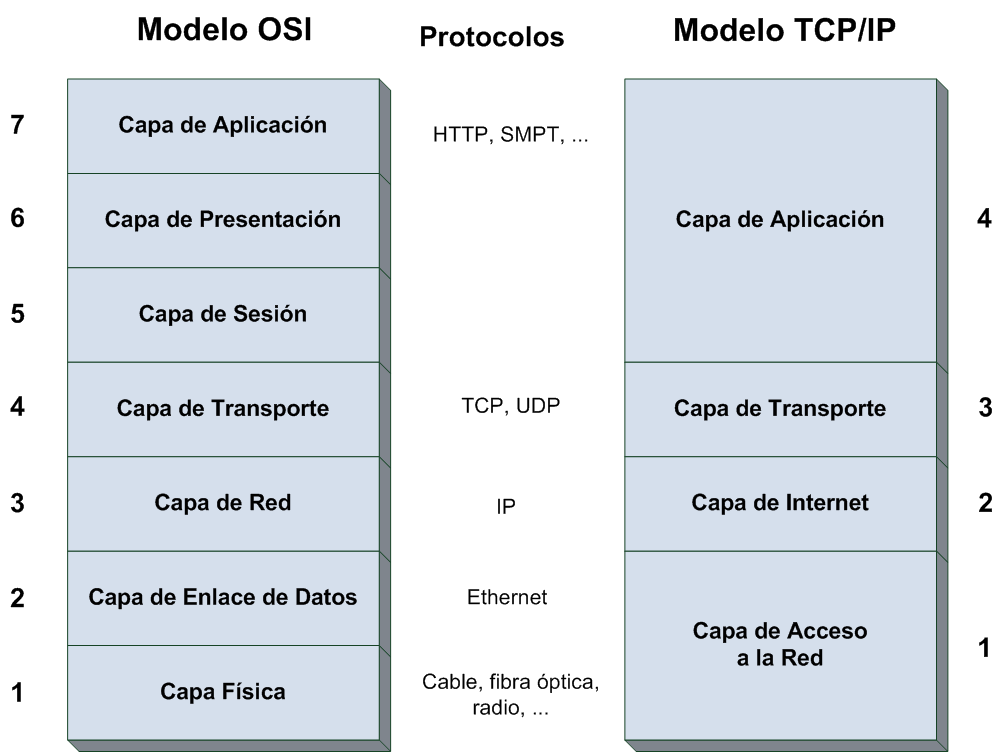
\includegraphics[width=0.9\textwidth]{imagenes/capas.png}
  \centering
  \caption{Modelos de capas de Internet.}
\end{figure}

\intro Dentro del modelo TCP/IP, que es el que se seguirá en este proyecto, es importante tener claro las siguientes 
capas, pues forma parte de los conocimientos básicos para lograr entender el emparejamiento de flujos.

\begin{itemize}

\item \textbf{Capa de aplicación}

En la capa de aplicación se encontrarán las aplicaciones de red y sus protocolos. 
Los protocolos que se encuentran en esta capa son HTTP, SMTP y FTP.

\begin{itemize}
\item El protocolo \textit{HTTP} permite la solicitud y transferencia de documentos web.
\item El protocolo \textit{SMTP} permite la transferencia de mensajes de correo electrónico.
\item El protocolo \textit{FTP} permite la transferencia de archivos entre dos terminales.
\end{itemize}

A parte de estos protocolos también corresponde a esta capa el \textbf{DNS}, el cual se encarga 
de traducir los nombres de los sitios web. 

\intro Para una información más extensa sobre la capa de aplicación consulte \cite{redes2010b}

\item \textbf{Capa de transporte}

La capa de transporte es la encargada de transportar los mensajes de la capa de aplicación. 
Los protocolos de esta capa son \textbf{TCP y UDP}. La principal diferencia y será algo que 
siempre se debe de tener presente cuando se trabaja con redes es que \textit{TCP} está orientado 
a garantizar la conexión, mientras que \textit{UDP} no garantiza la conexión.
\intro Para ampliar información sobre esta capa consulte \cite{redes2010c}

\begin{figure}[H]
  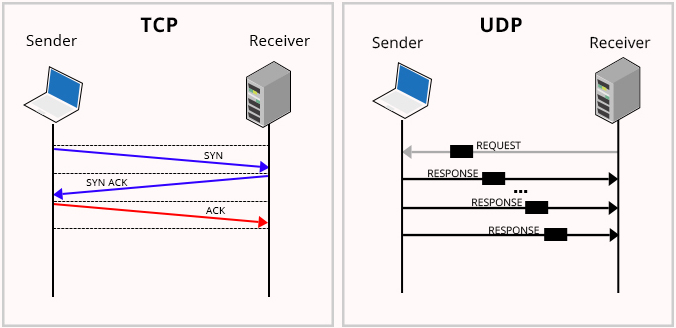
\includegraphics[width=1\textwidth]{imagenes/tcpudp.jpeg}
  \centering
  \caption{Diagrama de conexión de TCP y UDP.}
\end{figure}

\item \textbf{Capa de red}

En la capa de red es donde se encuentra el protocolo \textbf{IP}, el cual es el encargado de especificar 
el formato de envío entre los routers y los hosts y también el protocolo \textbf{ICMP}, el cual 
es un protocolo de control.

\intro En esencia, esta capa es la que se encarga de transportar los \textit{datagramas} de un \textit{host} a otro.

\intro Para ampliar sus conocimientos sobre la capa de red consulte \cite{redes2010d}

\end{itemize}

\intro En Internet la información que se envía se divide en paquetes. Estos paquetes tienen una IP de 
origen y otra de destino, así como un puerto de origen y un puerto de destino. Estos paquetes, que contienen 
parte de la información que se envía por la red, son unidos de nuevo una vez que llegan a su destino, de forma 
que entonces se dispondrá de la información completa. Dependiendo del tipo de protocolo se tolerarán perdidas 
de paquetes o no, para ilustrar esta idea, en una llamada mediante \textit{Skype} se tolera 
perder algunos paquetes, pues no se notará mucha diferencia. Si se pierden muchos paquetes 
la imagen se verá borrosa y la voz no se escuchará bien. Ahora en un correo electrónico, 
no se tolerará perder paquetes, pues entonces no se obtendrá la información completa. Cuando 
varios paquetes tienen el mismo origen y el mismo destino se denomina flujo. \cite{redes2010a}

\intro De esta forma se llega al emparejamiento de flujos, el cual es muy útil para los NMS, 
sistemas de monitoreo de red, \textit{Network Monitoring System}, como podría ser BRO \cite{broindex}.
Gracias al uso de estos programas el administrador de sistemas podrá prevenir ataques, como por ejemplo, los 
de denegación de servicio, DDoS, \textit{Distributed Denial of Service} \cite{redes2010e}. Un administrador 
de sistemas deberá de garantizar que el recurso que facilita y gestiona esté operativo siempre, 
por lo tanto analizará el tráfico para evitar los posibles ataques, virus, etc.

\intro Existen otras técnicas de clasificación de tráfico, como se puede ver en el artículo del 
departamento \citep{comparacion}, estas técnicas son: 

\begin{itemize}
\item Clasificación basada en los puertos de la capa de transporte. \cite{iana}
\item Clasificación basada en el contenido del paquete. \cite{payload}
\item Clasificación basada en la aplicación de técnicas de aprendizaje automático sobre estadísticas 
de tráfico. \cite{learning}
\end{itemize}

Hoy en día, las dos primeras técnicas mencionadas no son muy eficaces, pues por ejemplo:
\begin{itemize}
\item La primera técnica puede ser burlada fácilmente, haciendo que las conexiones pasen por el puerto 80.
\item En la segunda técnica, al tener que acceder a los paquetes, solo bastará con que estos estén 
encriptados para que no se pueda acceder a dicho paquete. Y también se debe de tener en cuenta que 
al acceder a los paquetes de una red que no es del propietario de la información es un delito y no respeta 
la privacidad.
\end{itemize}
\intro Ahora bien, la tercera técnica si es eficaz y fiable, pero su principal inconveniente es que 
necesita cierto tiempo para aprender a clasificar de una forma correcta el tráfico.

\intro Por lo tanto es necesario un nuevo método de clasificación, que sea funcional en cualquier circunstancia 
y sea eficiente desde el principio. Por ello, el método de emparejamiento planteado por el 
departamento \cite{comparacion} es muy atractivo al ser necesario saber solo las IP's y los puertos, 
ya que se respeta la seguridad, pues no es necesario acceder a los paquetes para conocer estos detalles. Incluso 
no sería necesario ser un proveedor de servicios de Internet, ISP, para conocer estos datos.


\section{Objetivos}

El objetivo de este trabajo es el desarrollo de un módulo para un NMS. Con el desarrollo del módulo se tratará 
de demostrar que el emparejamiento de flujos se puede realizar fuera de un entorno de laboratorio.

\begin{itemize}
\item Para ello será necesario conocer como Bro gestiona los flujos, desde su nacimiento a su muerte. 
\item También hará falta gestionar las entradas y salidas, aunque al principio se hará uso de un 
archivo \textit{pcap} de prueba para controlar si todo funciona bien, pudiendo pasar luego a analizar 
el tráfico de una red online.
\item Implementar la función de emparejamiento de flujos.
\item Será necesario realizar pruebas al módulo que se pretende desarrollar, de modo que se detecten los 
errores y se subsanen.
\end{itemize}

\intro Por último, y fuera de los objetivos más técnicos, el desarrollo de esta memoria también se 
considera un objetivo, que se tendrá en cuenta dentro de la temporización.

\section{Metodología}

Para realizar este trabajo se establecen una serie de tareas:

\begin{itemize}
\item Estado del Arte.
	\begin{itemize}
	\item Lectura del artículo del departamento. \cite{comparacion}
	\item Búsqueda de información sobre la identificación de tráfico.
	\end{itemize}
\item Análisis de las herramientas.
\item Diseñar el módulo de Bro.
\item Implementar el módulo.
\item Evaluación y pruebas del módulo.
\end{itemize}

%Cada tarea anterior se realimentará de la siguiente, el ejemplo más claro es el desarrollo del módulo, que 
%irá cambiando por las pruebas, pues se detectarán los fallos, a su vez habrá que releer el artículo mientras 
%se desarrolla el módulo para asegurarse de que todo se realiza de acuerdo al trabajo previo, etc.

\intro En el siguiente diagrama de Gantt se puede ver una temporización de estas tareas. 

\begin{figure}[H]
  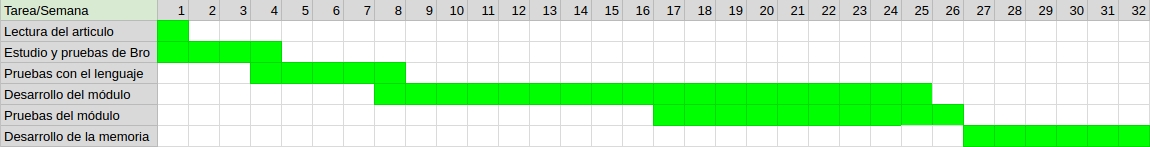
\includegraphics[width=1\textwidth]{imagenes/temporizacion.png} 
  \centering
  \caption{Temporización en diagrama de Gantt.}
\end{figure}

Este proyecto no necesita de ningún gasto, pues Bro \cite{broindex} proporciona sus binarios de 
forma gratuita. El módulo será subido a GitHub \cite{repo} con licencia de software libre, por lo que cualquiera 
podrá usarlo o modificarlo en el futuro. El único \textit{gasto} es el de un ordenador con Linux, 
o bien con Mac OS X, pues de momento no está disponible para Windows. \cite{brodownload}

\section{Estructura de la memoria}

Esta memoria se organizará de la siguiente forma: 
\begin{itemize}
\item En el capítulo 2 se hablará de todos los fundamentos teóricos y tecnológicos sobre los que se 
basa el proyecto.
\item En el capítulo 3 se contará cómo se pretende resolver el problema expuesto.
\item En el capítulo 4 se encontrará detallado cómo se han implementado los diferentes módulos.
\item En el capítulo 5 se realizarán las pruebas, para comprobar que todo funciona como 
estaba previsto, tanto a nivel funcional como a nivel de aplicación.
\item En el último capítulo se hablará de las conclusiones recogidas a lo largo de este proyecto y las posibles 
opciones que tiene para seguir trabajando sobre él.
\end{itemize}
\newpage